V této podkapitole se pustím do samotného testování objektových databází. Mezi testované databáze, které jsem pro účel své práce zvolil. Patří databáze DB4O, OrientDB a ObjectDB. Důvodem výběru těchto tří, byla dostupnost zdarma a aktivní vývoj. ObjectDB je sice komerční databáze, ale pro omezené potřeby (max 10 entitních tříd a 1 milión instancí entit) je možně ji využívat zcela bez poplatků.

Na následujících grafech jsou výsledky měření, veškeré hodnoty jsou v milisekundách.
\begin{figure}[!h]
\begin{subfigure}[b]{0.5\textwidth}
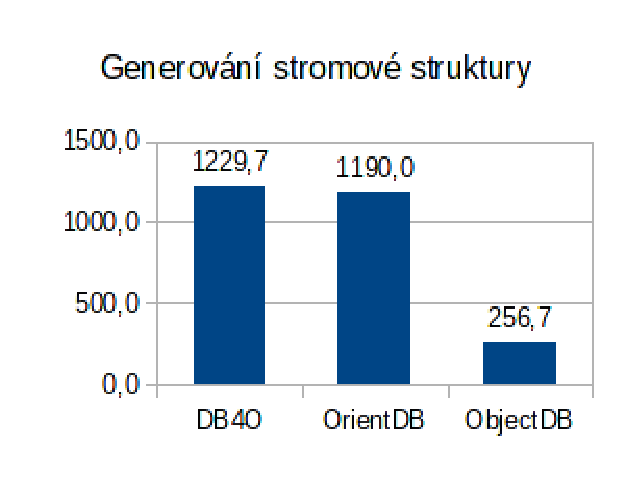
\includegraphics[width=20em]{obr/bench/oodbms1}
\end{subfigure}
\begin{subfigure}[b]{0.5\textwidth}
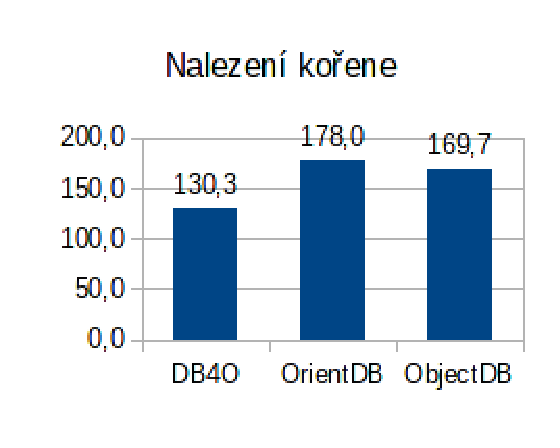
\includegraphics[width=20em]{obr/bench/oodbms2}
\end{subfigure}
\end{figure}


\begin{figure}[!h]
\begin{subfigure}[b]{0.5\textwidth}
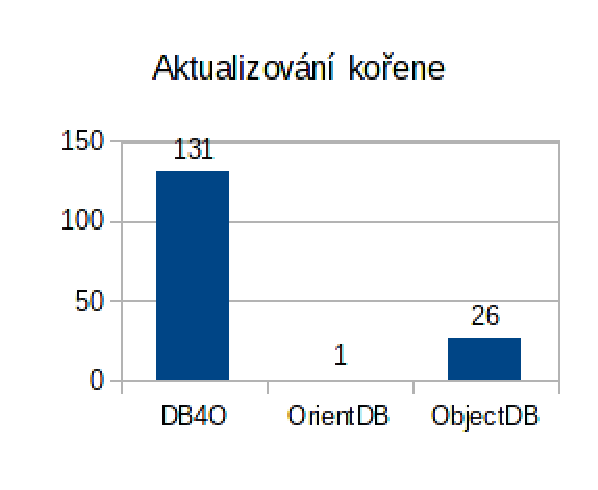
\includegraphics[width=20em, height=18em]{obr/bench/oodbms3}
\end{subfigure}
\begin{subfigure}[b]{0.5\textwidth}
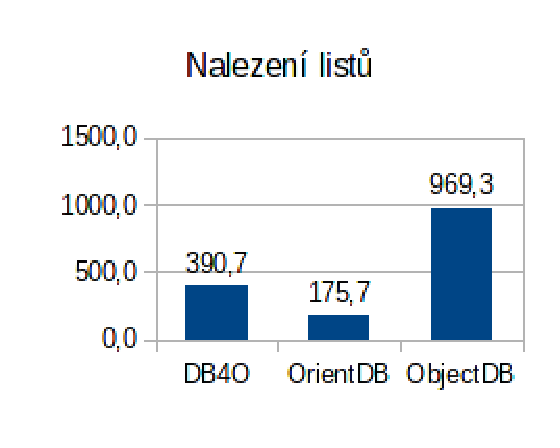
\includegraphics[width=20em, height=18em]{obr/bench/oodbms4}
\end{subfigure}
\begin{subfigure}[b]{0.5\textwidth}
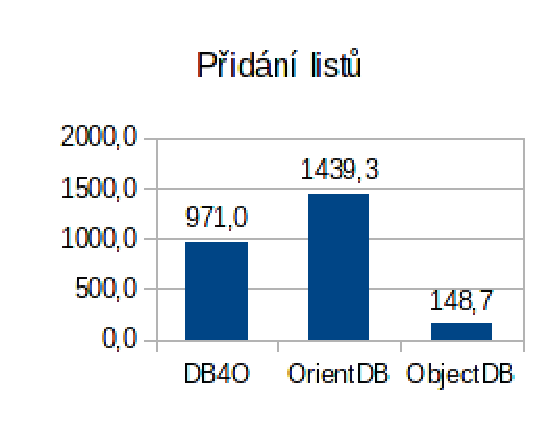
\includegraphics[width=20em, height=18em]{obr/bench/oodbms5}
\end{subfigure}
\begin{subfigure}[b]{0.5\textwidth}
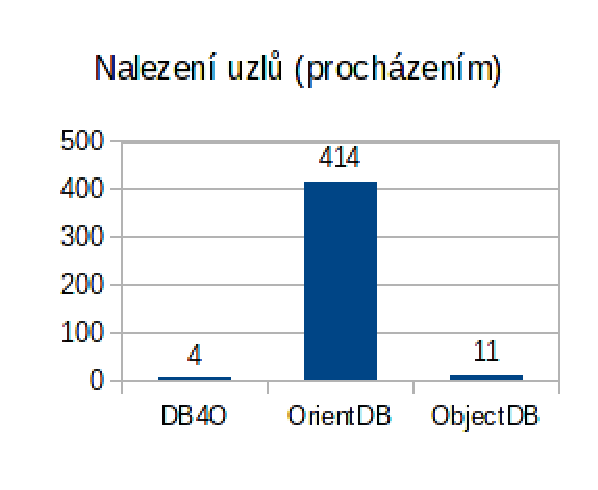
\includegraphics[width=20em, height=18em]{obr/bench/oodbms6}
\end{subfigure}
\begin{subfigure}[b]{0.5\textwidth}
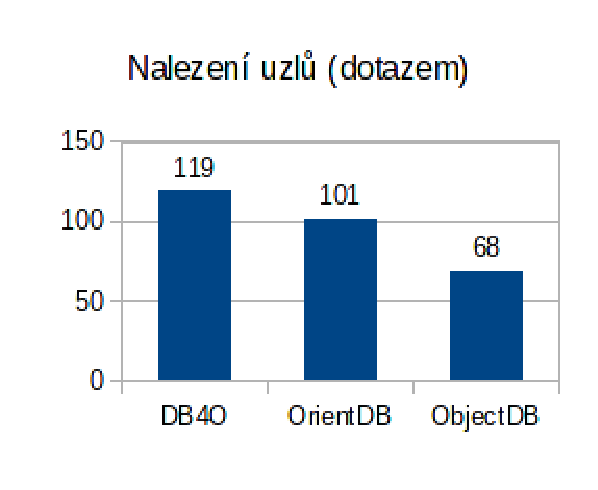
\includegraphics[width=20em, height=18em]{obr/bench/oodbms7}
\end{subfigure}
\begin{subfigure}[b]{0.5\textwidth}
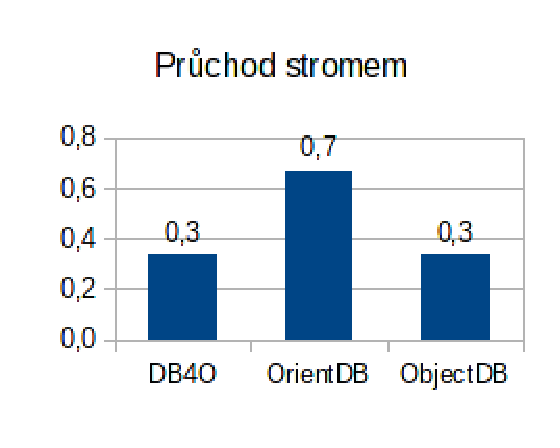
\includegraphics[width=20em, height=18em]{obr/bench/oodbms8}
\end{subfigure}
\end{figure}

\begin{figure}[!h]
\begin{subfigure}[b]{0.5\textwidth}
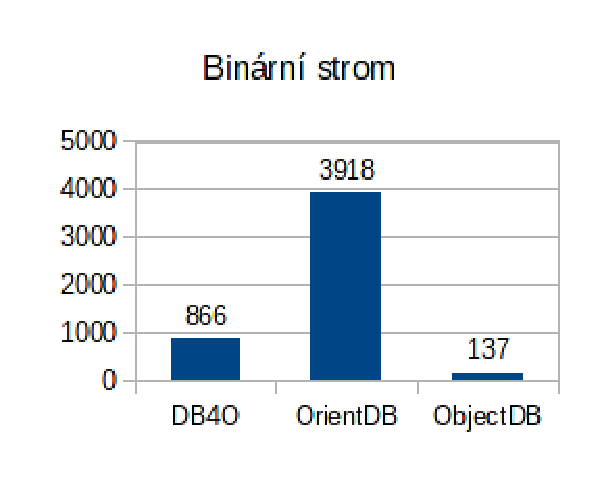
\includegraphics[width=20em]{obr/bench/oodbms9}
\end{subfigure}
\begin{subfigure}[b]{0.5\textwidth}
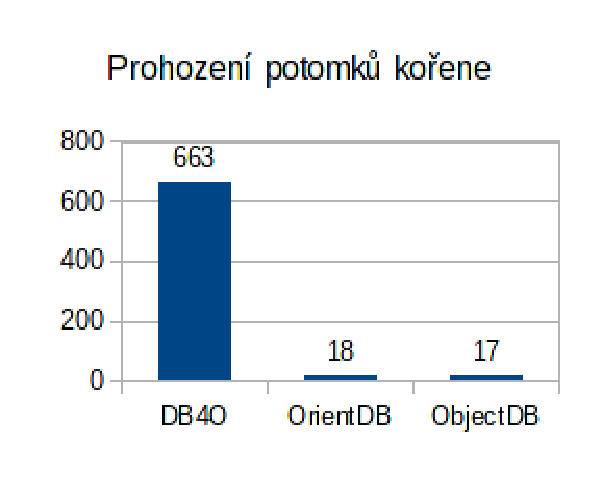
\includegraphics[width=20em]{obr/bench/oodbms10}
\end{subfigure}
\begin{subfigure}[b]{0.5\textwidth}
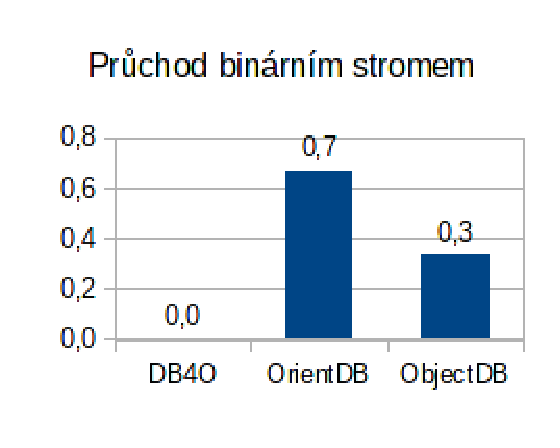
\includegraphics[width=20em]{obr/bench/oodbms11}
\end{subfigure}
\begin{subfigure}[b]{0.5\textwidth}
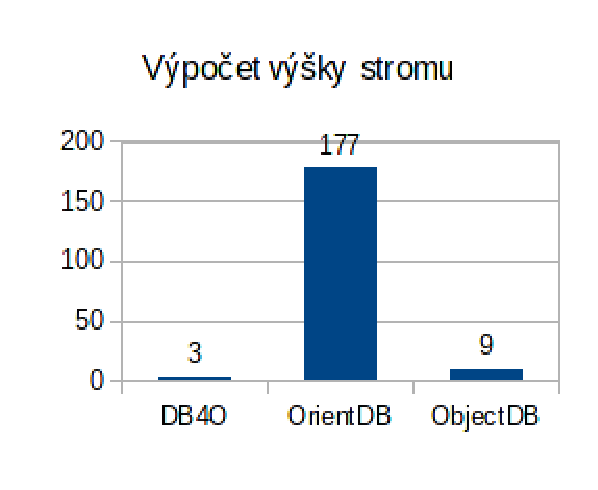
\includegraphics[width=20em]{obr/bench/oodbms12}
\end{subfigure}
\begin{subfigure}[b]{0.5\textwidth}
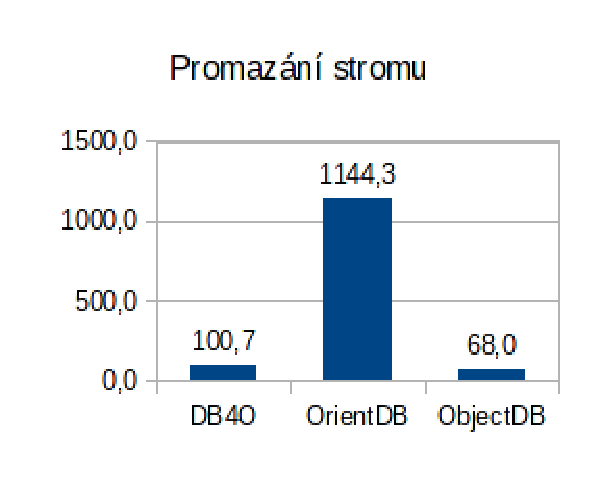
\includegraphics[width=20em]{obr/bench/oodbms13}
\end{subfigure}
\begin{subfigure}[b]{0.5\textwidth}
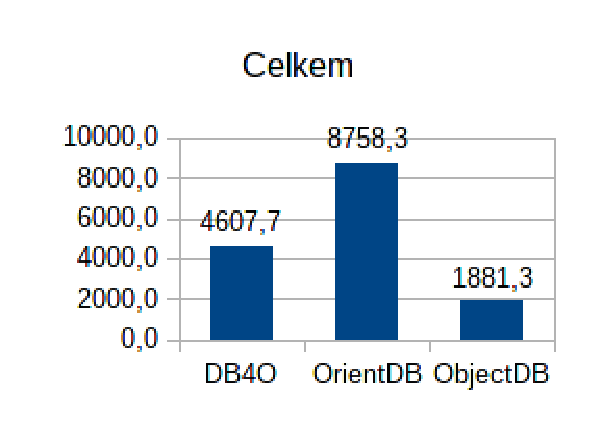
\includegraphics[width=20em]{obr/bench/oodbms14}
\end{subfigure}
\end{figure}


